\chapter{Konzepte}
\label{sec:konzepte}

In diesem Kapitel werden Konzepte beschrieben, die möglichst abstrakt gehalten sind. Entwickler (Besonders Anfänger) eines Online-Multiplayer Spiels sollen anhand von diesen Konzepten eine Hilfestellung bekommen, um einen roten Faden in ihrer Entwicklung verfolgen zu können. Insbesondere wenn der Entwickler noch wenig oder keine Erfahrung mit der Entwicklung von Online-Mulitplayerspielen gesammelt hat, sollen diese Konzepte bei der Erstellung einer soliden Grund-Architektur dienlich sein.

Bevor eines dieser Konzepte angewandt werden kann, müssen folgende Voraussetzungen erfüllt sein:

1. Das grundsätzliche Spielkonzept wurde erarbeitet und steht fest.

2. Anhand von dem festgelegten Spielkonzept kann abgeschätzt werden, ob sich für das Spiel eine Client / Server oder eine Client / Host Architektur eignet.

Sollte das Team bzw. der Solo-Entwickler zum Entschluss gekommen sein dass sich ein Client / Server Modell am besten für den spezifischen Use-Case eignet, so müssen Vorkehrungen getroffen werden, um die Hardware-Ressourcen für den späteren Server-Runner bzw. die Matchmaking API sicher zu stellen. Die Grundvoraussetzung ist jedoch ein aus dem Internet erreichbarer PC mit einer festen IP-Adresse. 

Alternativ kann auch zunächst lokal innerhalb eines LAN \cite{Wikipedia.2022} entwickelt werden. Hierbei ist jedoch wichtig, dass eventuell auftretende Seiteneffekte, die durch Latenz \cite{Wikipedia.2022b} oder Bandbreite \cite{Wikipedia.2019b} verursacht werden, nicht unter Realbedingungen getestet werden können. 

Es empfiehlt sich deshalb bereits innerhalb der ersten Entwicklungsiterationen auszutesten, wie Prototypen für Serverprozesse auf unterschiedliche Standorte der Serverhardware reagieren. 

Nun gilt es einen passenden Technologie-Stack zu finden. Hier gibt es keine Klare Empfehlung, jedoch können die in diesem Kapitel beschriebenen Konzepte als Entscheidungshilfe dienen. Auf dem offenen Markt existieren bereits Frameworks \& Game Engines, die Manche dieser Konzepte bereits implementiert haben und als Libraries für Entwickler bereitstellen.

\cite{MFatihMAR.2021}

\section{Vorwort zu den aufgestellten Konzepten}

Wie bereits in der Einführung erläutert, sind die folgenden Konzepte keine konkrete Entwicklungsanleitung. Viel mehr sind sie im Kontext einer bereits erarbeiteten Spielidee eine Hilfestellung zur Erarbeitung einer individuellen technischen Architektur.

Konkret muss beachtet werden, dass einige der Konzepte nicht als einzelne Programm-Klassen verstanden werden müssen, sondern als Hilfestellung für Ableitungen zu konkreten Klassen oder Skripten genutzt werden können. Es ist auch gut denkbar, dass einige Implementierungen deutliche Vorteile genießen, wenn bestimmte Konzepte jeweils für getrennte Spiel-Szenen \cite{Wikipedia.2012} umgesetzt werden.

Die Konzepte sind als separat voneinander zu betrachtende Softwarekomponenten zu sehen, die miteinander kommunizieren können. Man könnte die einzelnen implementierten Konzepte auch als Microservices \cite{Thones.2015} bezeichnen, die innerhalb eines Server-Prozesses eigene interne Abläufe besitzen und durchführen. Die Kommunikation zwischen den Komponenten sollte über direkte gegenseitige Funktionsaufrufe oder über Event-gesteuerte Funktionen \cite{Michelson.2006} geschehen.

\section{API für Matchmaking \& Server Runner}

Bei diesem Konzept muss eine API entworfen werden, welche unabhängig von einem existierenden Client oder Serverprozess arbeitet. Diese API hat 2 grundsätzliche Aufgaben. 

Matchmaking:

Die API muss einen Algorithmus implementieren, welcher mehrere Spieler zu einer Spiel-Session zusammenführt. Mögliche Matchmaking Konzepte sind bereits im Hintergrund-Kapitel beschrieben. Die Matchnaking API verwaltet als eine Liste an aktiven Serverprozessen sowie die Information, wie man sich zu ihnen verbindet. In der Regel wird pro Serverprozess ein Netzwerk-Port an der Server-Maschine reserviert, auf denen sich dann N Spieler verbinden können.

Je nach Spielkonzept können hunderte, tausende Serverprozesse existieren, welche jeweils nur eine vergleichsweise geringe Anzahl (1-20) an Spieler verwalten. Spielkonzepte, welche viele Spieler (200-1000) innerhalb eines einzigen Serverprozesses voraussetzten, erzeugen dagegen zwar quantitativ weniger Serverprozesse, diese neigen aber in der Regel schnell zu Überlastung. Neben der Umsetzung von Interest Management und einer schlanken Architektur für möglichst wenig Network-Traffic kann aber auch die Matchmaking API Abhilfe schaffen, bspw. durch "Umverlegung" von Spielern auf andere oder neue Serverprozesse.

Server Runner:

Neben dem Matchmaking ist die API ebenfalls auch zuständig für das Starten und die Überwachung von Serverprozessen.
Ebenfalls können technische Statusinformationen über aktuell laufende Spiel innerhalb eines Serverprozesses von der API verwaltet werden (Bspw. ob es möglich ist einem Server beizutreten, oder wieviele Spieler bereits auf einem Serverprozess spielen)

\begin{figure}
	\centering
	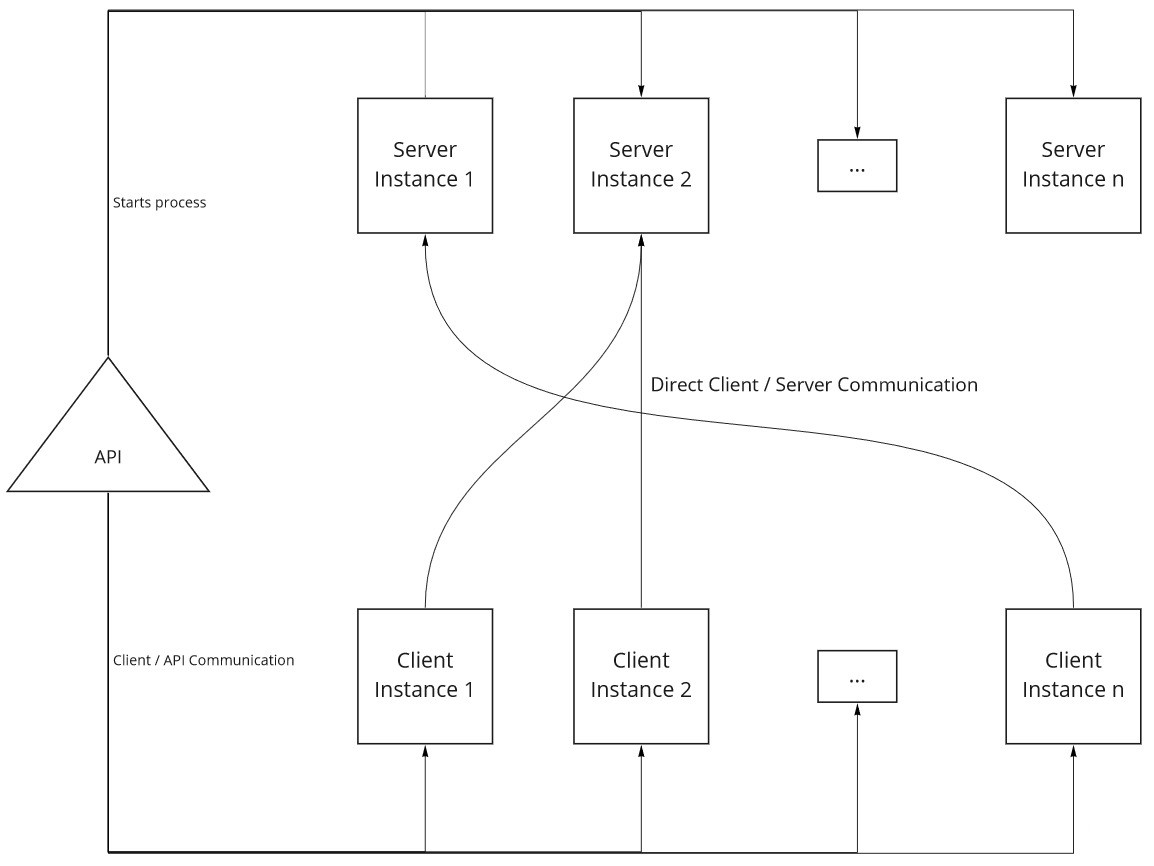
\includegraphics[width=150mm]{images/API_Konzept_Diagramm.jpg}
	\caption[API Konzept Diagramm]{Veranschaulichung des API Konzepts}
	\label{pic:API_Konzept_Diagramm}
\end{figure}


Je nach Use-Case kann das Aufgabenfeld der API um weitere Punkte erweitert werden, hier ein paar Beispiele:
- Datenbank für Authentifizierung bzw. Kommunikation mit externen SSO-Service Providern \cite{Wikipedia.2021c} 
- Datenbank für InGame Shop / Kommunikation mit externen Lösungen

\section{Client UI \& Visual Controller}

Das Konzepts des Client UI \& Visual Controllers beschreibt die Art und Weise, wie die Benutzeroberfläche und visuelle Ebene eines Spielers durch Antworten des Servers oder einzelner Spieleraktivitäten manipuliert wird.

\begin{figure}
	\centering
	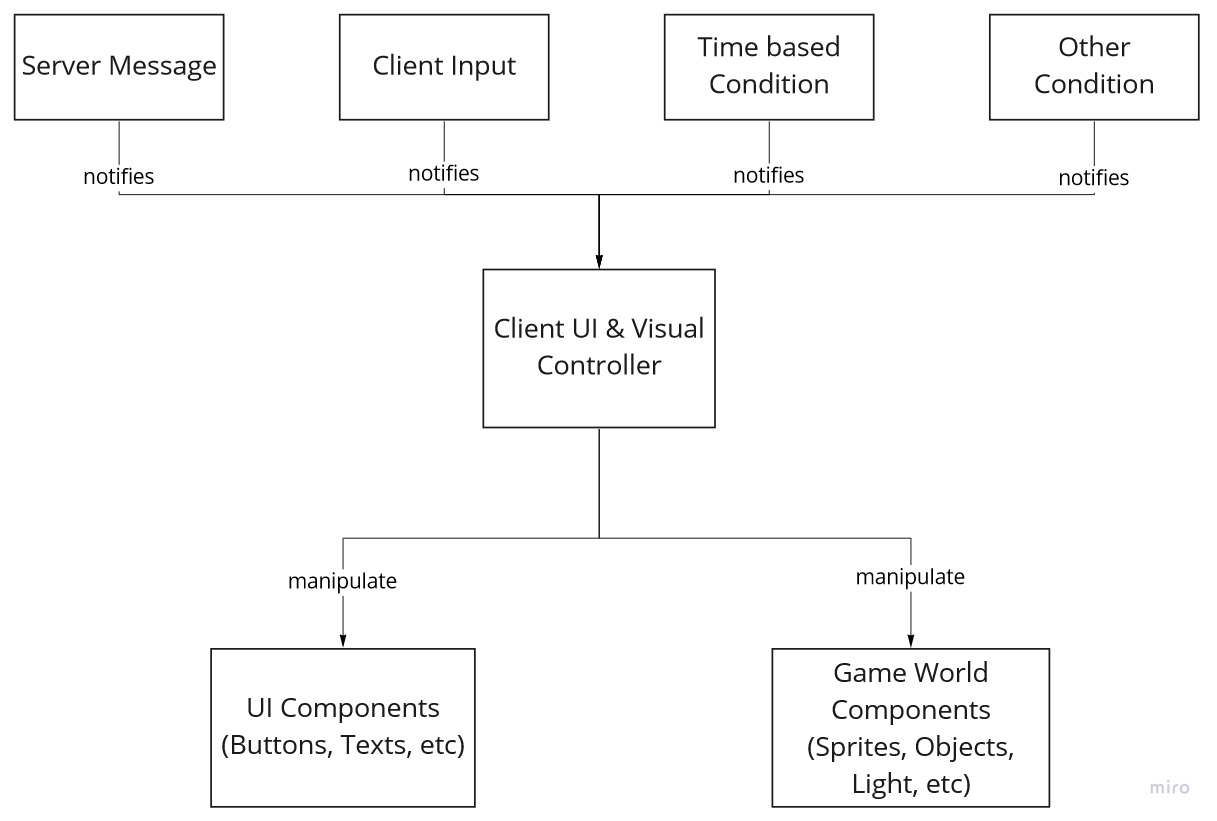
\includegraphics[width=150mm]{images/Client_UI_und_Visual_Konzept.jpg}
	\caption[Client UI \& Visual Controller Diagramm]{Veranschaulichung des Client UI \& Visual Controller Konzepts}
	\label{pic:Client_UI_und_Visual_Konzept}
\end{figure}

Konkret sorgt ein Server-Ereignis, der Input eines Spielers (beispielsweise durch klicken eines Buttons oder einsammeln eines Gegenstands) oder eine andere Bedingung dafür, dass Funktionen innerhalb des Client UI \& Visual Controllers aufgerufen werden. Innerhalb dieser Funktionen werden Komponenten der Benutzeroberfläche wie z.b. Anzeigetexte, Bilder etc. oder Objekte innerhalb der Spielwelt selbst manipuliert.

Wichtig ist, dass Funktionen des Client UI \& Visual Controller erst nach server- oder clientseitigen Überprüfungen ausgeführt werden. Der Controller selbst sollte nur überprüfen, ob fluktuierende Komponenten noch existieren oder sich in einem konsistenten Zustand befinden. Spielrelevante Logik, beispielsweise ob ein Spieler berechtigt ist, bestimmte Aktionen durchzuführen, ist nicht Teil des Client UI \& Visual Controllers.

\section{Server Network Manager}

Der Server Network Manager ist für die korrekte Abarbeitung von serverseitigen Aufgaben zuständig, welche aufkommen, sobald ein Netzwerk-spezifisches Ereignis stattfindet.

Beispiel: Die Verbindung eines Clients bricht mitten in der Laufenden Spielszene ab. Der Server Network Manager stößt nun Funktionen anderer serverseitigen Manager-Komponenten an, welche dafür sorgen, dass alle Spieler über den neuen Zustand des Spiels informiert werden. Hierfür müssen zunächst serverinterne Variablen aktualisiert werden.

Beispiel: In einem Online-Ableger des Spiels "Mensch ärger dich nicht" verliert ein Spieler seine Netzwerk-Verbindung. Nun muss der Server Network Manager dafür sorgen, dass das Spiel trotzdem zuende gespielt werden kann. Die gespawnten Spielfiguren des ausgeschiedenen Spielers müssen entfernt, und der Spiel-Fortschritt aktualisiert werden. Diese Funktionen stellt möglicherweise der \hyperref[spawn_manager]{Runtime Spawn Manager}, \hyperref[progress_manager]{Progress / Game State Manager } zur Verfügung.
Außerdem muss dem \hyperref[serverside_client_manager]{Serverside Client Manager} mitgeteilt werden, dass dieser Spieler nun nicht mehr Teil der Spiel-Session ist.


\begin{figure}
	\centering
	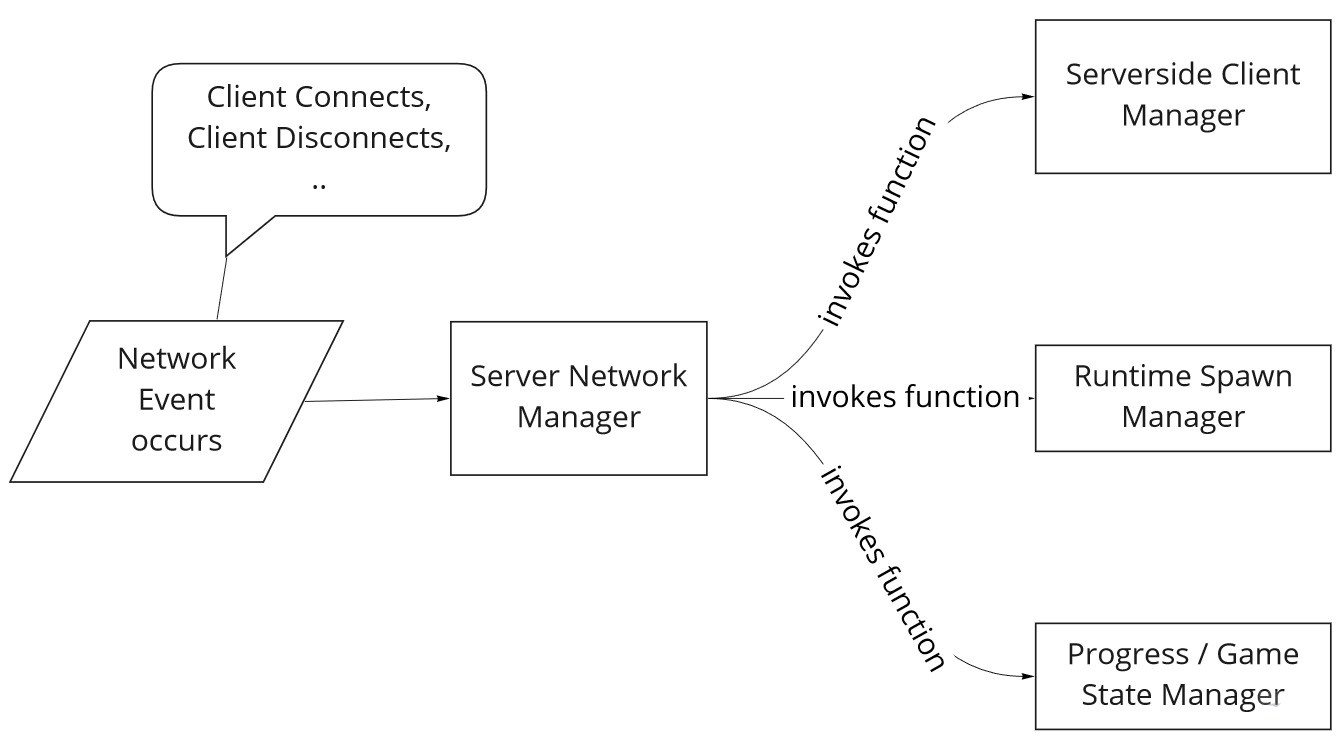
\includegraphics[width=150mm]{images/Server_Network_Manager.jpg}
	\caption[Server Network Manager Diagramm]{Veranschaulichung des Server Network Manager Konzepts}
	\label{pic:Server_Network_Manager}
\end{figure}


\section{Lobby / Multi Scene Manager (optional)}

Dieses Konzept lässt sich nur dann anwenden, wenn das Spielkonzept mehrere, von einander unabhängige Spiel-Szenen voraussetzt (Bsp. Menü-Szene, Lobby-Szene, Spiel-Szene).  

Der Lobby/ Multi Scene Manager ist eine serverseitige Komponente, welche es erlaubt, Spielszenen-übergreifende Informationen zu speichern und zu verwalten. Beispielsweise könnte bei einem Lobby-basierten Matchmaking die Information des Leiters einer Lobby über Spielszenen hinweg gespeichert werden. Ebenso wäre es denkbar, dass der Bereitschafts-Status vor dem tatsächlichen Spiel innerhalb des Lobby / Multi Scene Managers gespeichert wird.

Außerdem stellt der Lobby / Multi Scene Manager Funktionen bereit, welche
- alle Clients informiert, sobald ein globaler Szenenwechsel angestoßen werden soll
- alle Clients über den aktuellen Status einer Lobby informiert.

\begin{figure}
	\centering
	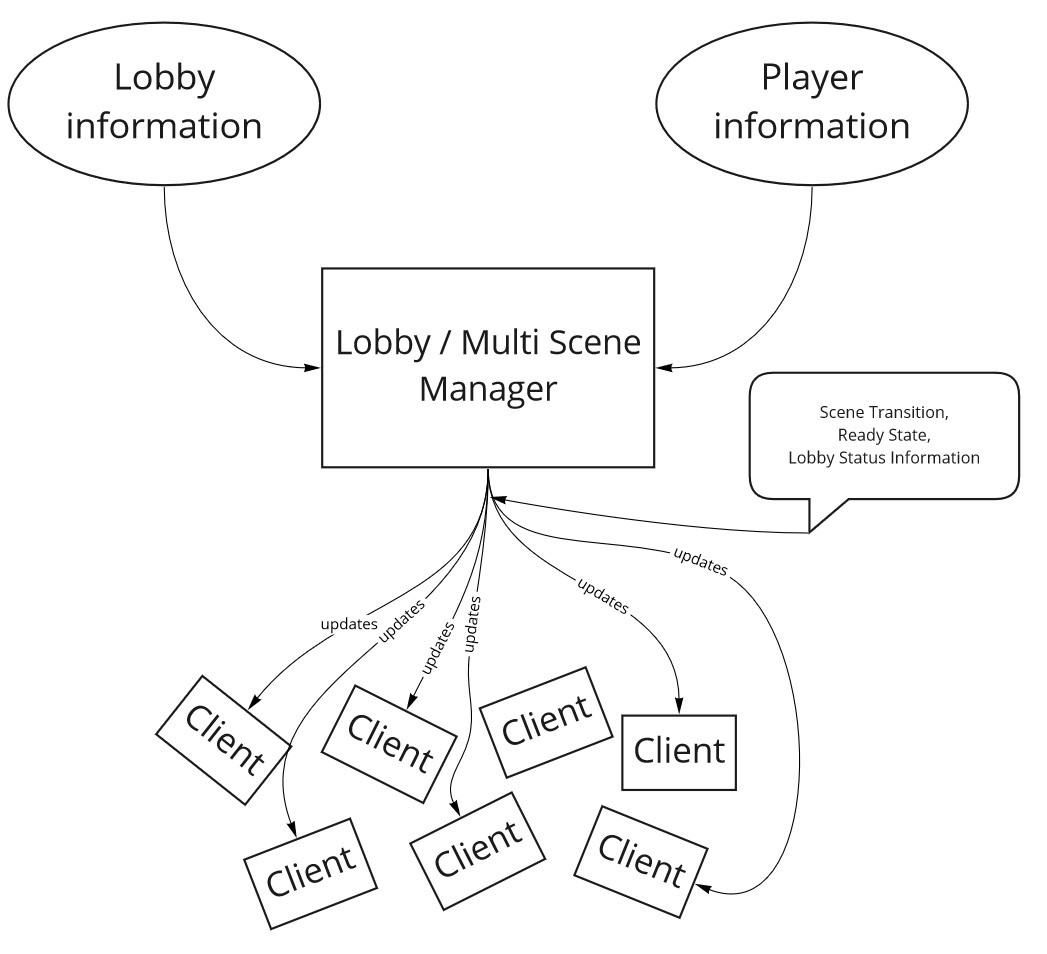
\includegraphics[width=150mm]{images/Lobby_Multi_Scene_Manager.jpg}
	\caption[Lobby / Mutli Scene Manager Diagramm]{Veranschaulichung des Lobby / Mutli Scene Manager Konzepts}
	\label{pic:Lobby_Multi_Scene_Manager}
\end{figure}


\section{Client Connection Manager}

Das Konzept Client Connection Manager beschreibt eine Softwarekomponente, welche folgende Aufgaben umsetzen muss:

- Implementierung von clientseitigen Methoden zum Informationsaustausch mit Matchmaking API.
Z.B. stellt die Matchmaking API dem Client über HTTP-Kommunikation Informationen bereit, mit denen sich der Client auf einen speziellen Server verbinden kann (IP + Port). \cite{Wikipedia.2021d} \cite{Wikipedia.2021e}

- Verarbeitung der von Matchmaking API bereitgestellten Informationen. 

Z.B. könnte die Matchmaking API einem Client die Information bereit stellen, dass aus einem bestimmten Grund dem angeforderten Serverbeitritt verweigert wird. Diese Information muss der Client Connection Manager "Zwischenspeichern" und verwalten.

- Aufruf von Methoden eines Client UI Controllers.

Z.B. Die soeben erlangte Information über den verweigerten Serverbeitritt muss nun dem Nutzer dargestellt werden, hierfür ruft der Client Connection Manager Funktionen auf, welche ein Client UI Controller implementiert hat.

- Bereitstellung von Funktionen, welche den Beitritt zu einem Game-Server sicherstellen.

- Ausführen von Handler-Funktionen und Auslösen von Callbacks für clientseitige Konsequenzen bei Netzwerkabbruch, manuellem Verlassen einer Server-Session oder sonstigen Abbruchgründen, welche dazu führen, dass eine Online-Spielsession verlassen wird.

Z.B. Wird die notwendige Verbindung zum Internet während des Spiels unterbrochen. Der Client Connection Manager löst Callbacks aus, welche im Client UI \& Visual Controller implementiert sind. Diese Sorgen dafür, dass der Spieler zurück ins Hauptmenü geleitet wird, in dem eine Fehlermeldung dargestellt wird, welche erklärt warum das Spiel abgebrochen ist.

\begin{figure}
	\centering
	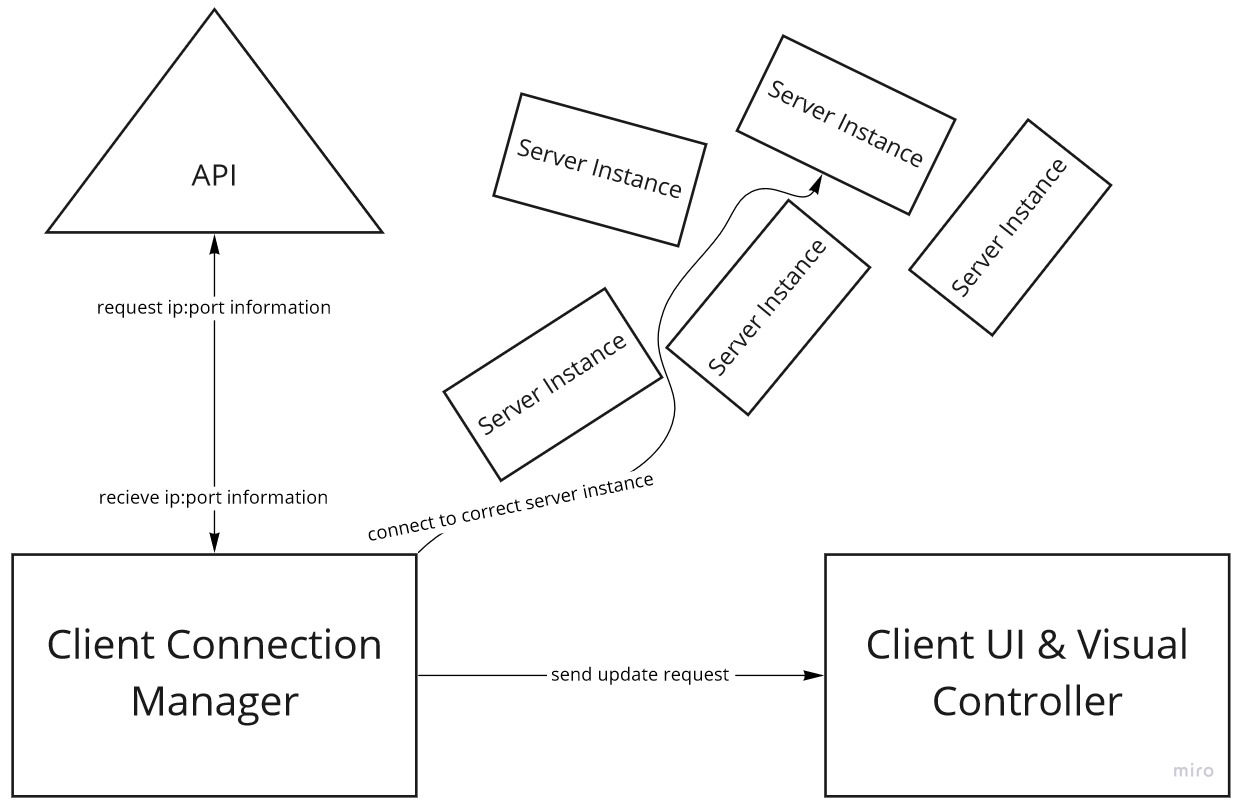
\includegraphics[width=150mm]{images/Client_Connection_Manager.jpg}
	\caption[Client Connection Manager Diagramm]{Veranschaulichung des Client Connection Manager Konzepts}
	\label{pic:Client_Connection_Manager}
\end{figure}



\section{Serverside Client Manager}

\label{serverside_client_manager}

Das Konzept des serverseitigen Client Manager beinhaltet die Verwaltung aller verbundener Clients innerhalb eines aktiven Serverprozesses. Insbesondere speichert der serverseitige Client Manager 2 Arten von Information über jeden Client:

Einerseits werden Netzwerk-bezogene Informationen über einen Client gespeichert, im einfachsten Fall ist dies lediglich die IP Adresse des Hosts sowie der Port, auf welchem der Server seinen Kommunikationskanal geöffnet hat. Bei Spielkonzepten, welche eine weitergehende Authentifizierung des Spielers voraussetzen, können hier auch Benutzernamen, Benutzertags, Email-Adressen o.ä. gespeichert und weiterverarbeitet werden.

Zum Anderen speichert und verwaltet der serverseitige Client Manager auch spielspezifische Informationen wie Bspw. den aktuellen Anzeigenamen, konfigurierte Individualisierung des Spielcharakters, Spielerrollen oder andere Eigenschaften, über die der Server während einer Spiel-Session Kenntnis haben sollte.

\begin{figure}
	\centering
	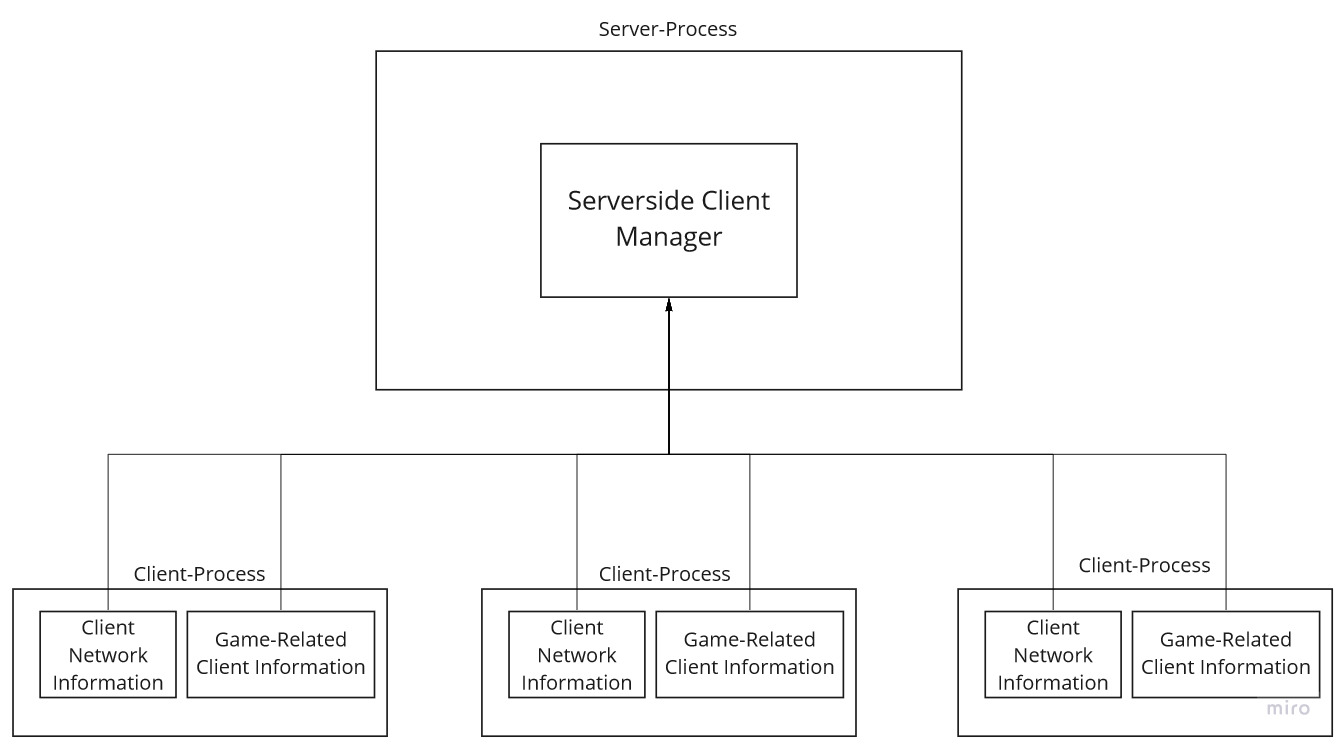
\includegraphics[width=150mm]{images/serversided_client_manager.jpg}
	\caption[Serversided Client Manager]{Veranschaulichung des serverseitigen Client Manager Konzepts}
	\label{pic:serversided_client_manager}
\end{figure}

\section{Prepare-Game-Manager}

Der Prepare-Game-Manager ist Teil des Serverprozesses und beinhaltet alle Funktionen, welche nötig sind um eine Spielszene vorzubereiten, bevor die Spieler ihr beitreten dürfen. Die Funktionen sollten konkret umsetzen:

- Spawning \cite{Wikipedia.2020} von NPCs \cite{Wikipedia.2021f} oder Spielgegenständen, die in Abhängigkeit zur Anzahl der beitretenden Spieler, einer Spielkonfiguration oder sonstigen Parametern stehen.

- Anpassung der Eigenschaften von bereits gespawnten NPCs oder Spielgegenständen, die in Abhängigkeit zur Anzahl der beitretenden Spieler, einer Spielkonfiguration oder sonstigen Parametern stehen.

- Initialisierung der Spawnpunkte für Spieler anhand von Spawnalgorithmen oder festgelegten Punkten in der Spielwelt.

- Abarbeitung sonstiger serverseitigen Abläufe, welche Voraussetzung für den Start des Spiels sind

\begin{figure}
	\centering
	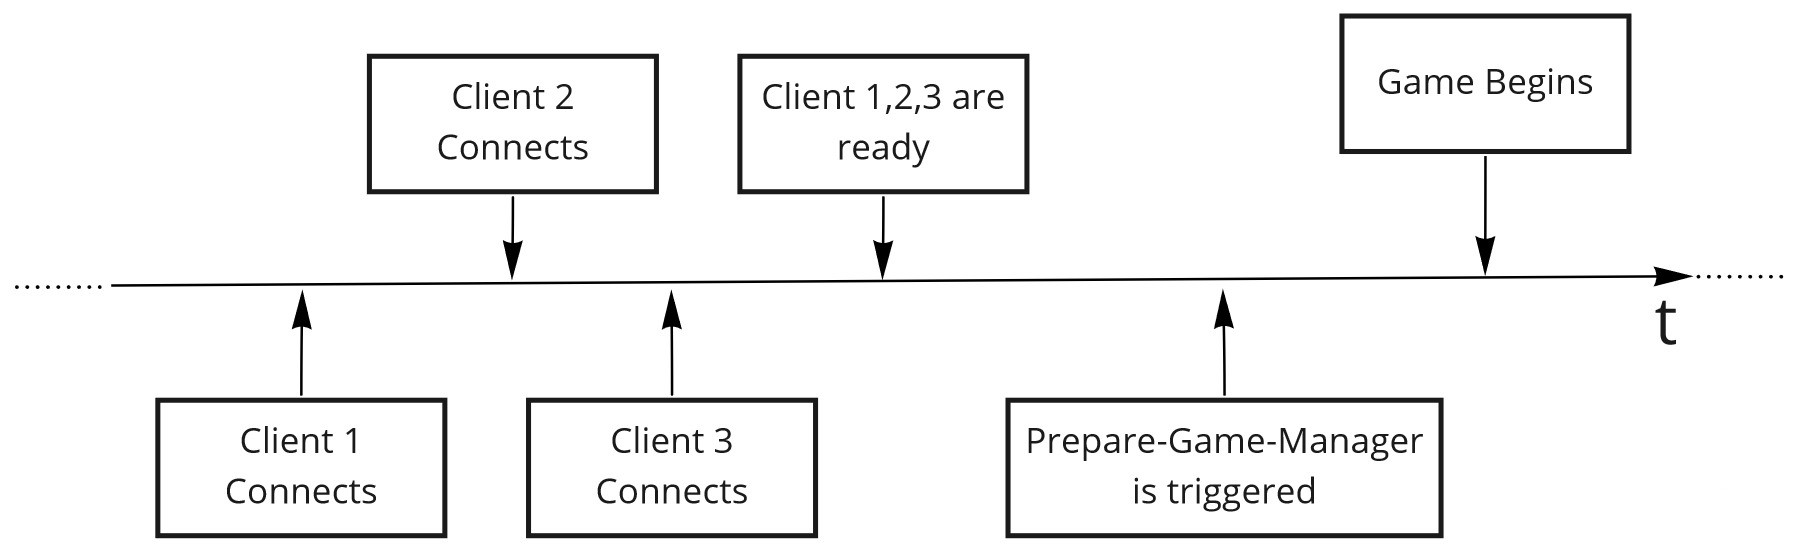
\includegraphics[width=150mm]{images/prepare_game_manager.jpg}
	\caption[Prepare-Game-Manager]{Veranschaulichung des Prepare Game Manager Konzepts}
	\label{pic:prepare_game_manager}
\end{figure}

\section{Progress / Game-State Manager}
\label{progress_manager}

Die Aufgabe eines Progress bzw. Game-State Managers ist es, Gewinn bzw. Verlustbedingungen einer Spielsession zu speichern und zu verwalten. 

Beispiele hierfür sind:
- Verwaltung und Synchronisierung von globalen Timern
- Verwaltung und Synchronisierung von Spiel-Kennzahlen (z.B. der Spielstand bei einem Fußball-Match)

Außerdem ist der Progress Manager / Game-State Manager dafür verantwortlich, alle Clients über spielentscheidende Ereignisse zu informieren. 

\begin{figure}
	\centering
	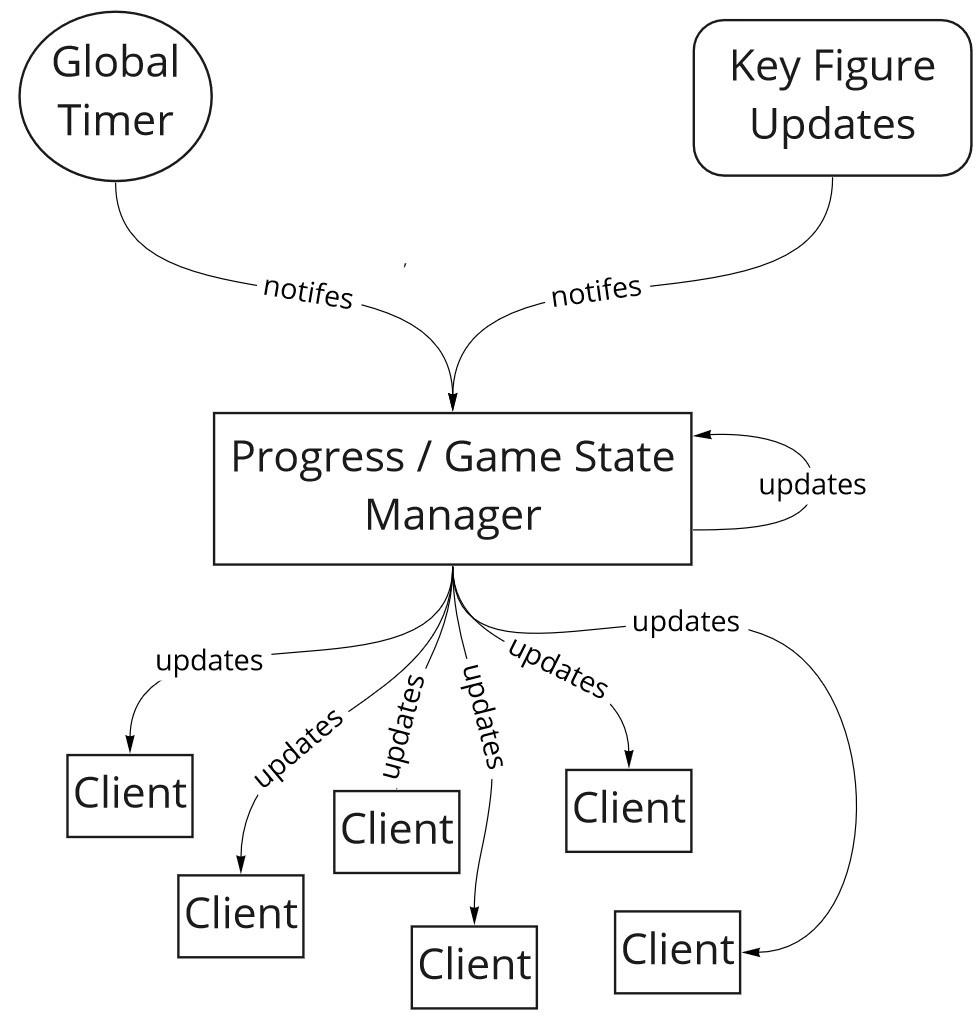
\includegraphics[width=150mm]{images/Progress_State_Manager.jpg}
	\caption[Progress / Game-State Manager]{Veranschaulichung des Progress / Game-State Manager Konzepts}
	\label{pic:Progress_State_Manager}
\end{figure}

\section{Runtime Spawn Manager}
\label{spawn_manager}

Der Runtime Spawn Manager verwaltet die zur Laufzeit zu erzeugenden Spieler und Nicht-Spieler Objekte. Konkret werden Funktionen des Runtime Spawn Managers ausgeführt, wenn ein spezifisches Event innerhalb einer Spiel-Session ausgelöst wird oder ein Spieler bzw. Nicht-Spieler-Character stirbt, und diese erneut an anderer Position spawnen sollen ("Re-Spawning"). Die Logik, wo genau ein Spieler oder Nicht-Spieler Objekt seine neue Einstiegsposition erhält, regelt ebenfalls der Runtime Spawn-Manager.

Ein Beispiel: In einem Online Multiplayer Ego-Shooter \cite{Wikipedia.2021g} stirbt ein Spieler durch Schüsse anderer Spieler. Der Runtime Spawn Manager sorgt dafür, dass anhand von bestimmten, zur Laufzeit ausgerechneten Bedingungen eine neue Spawn-Position für den gestorbenen Spieler gefunden wird. 

\begin{figure}
	\centering
	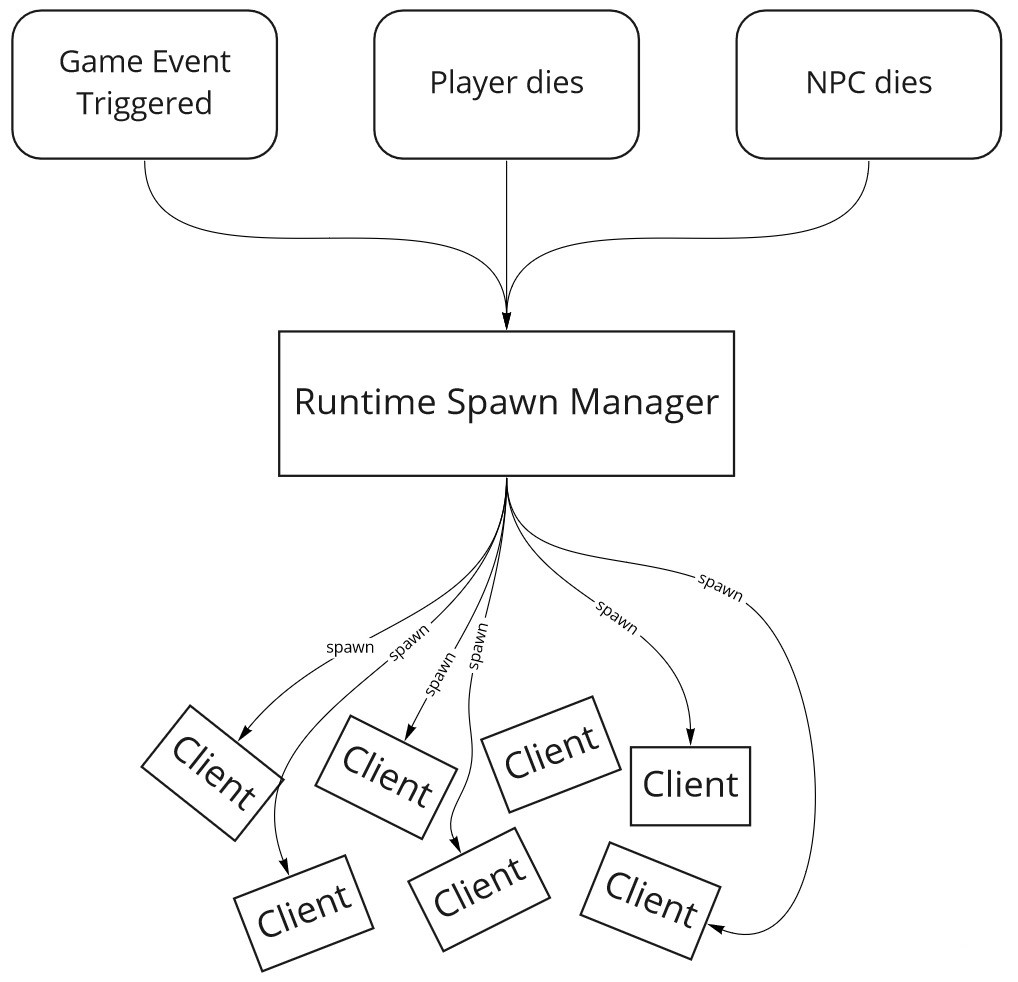
\includegraphics[width=150mm]{images/Runtime_Spawn_Manager.jpg}
	\caption[Runtime Spawn Manager]{Veranschaulichung des Runtime Spawn Manager Konzepts}
	\label{pic:Runtime_Spawn_Manager}
\end{figure}

\section{Interest Manager}

Wie bereits in der Sektion über \hyperref[interest_management]{Interest Management} erklärt, ist es je nach Spielkonzept notwendig, dass der Spieler stets nur über den für ihn relevanten Teil der Spielwelt Kenntnis hat. Aus diesem Grund sollten sich angehende Spieler-Entwickler fragen, ob sie eine solche Software-Komponente in die Architektur ihres Projekts integrieren möchten.

\begin{figure}
	\centering
	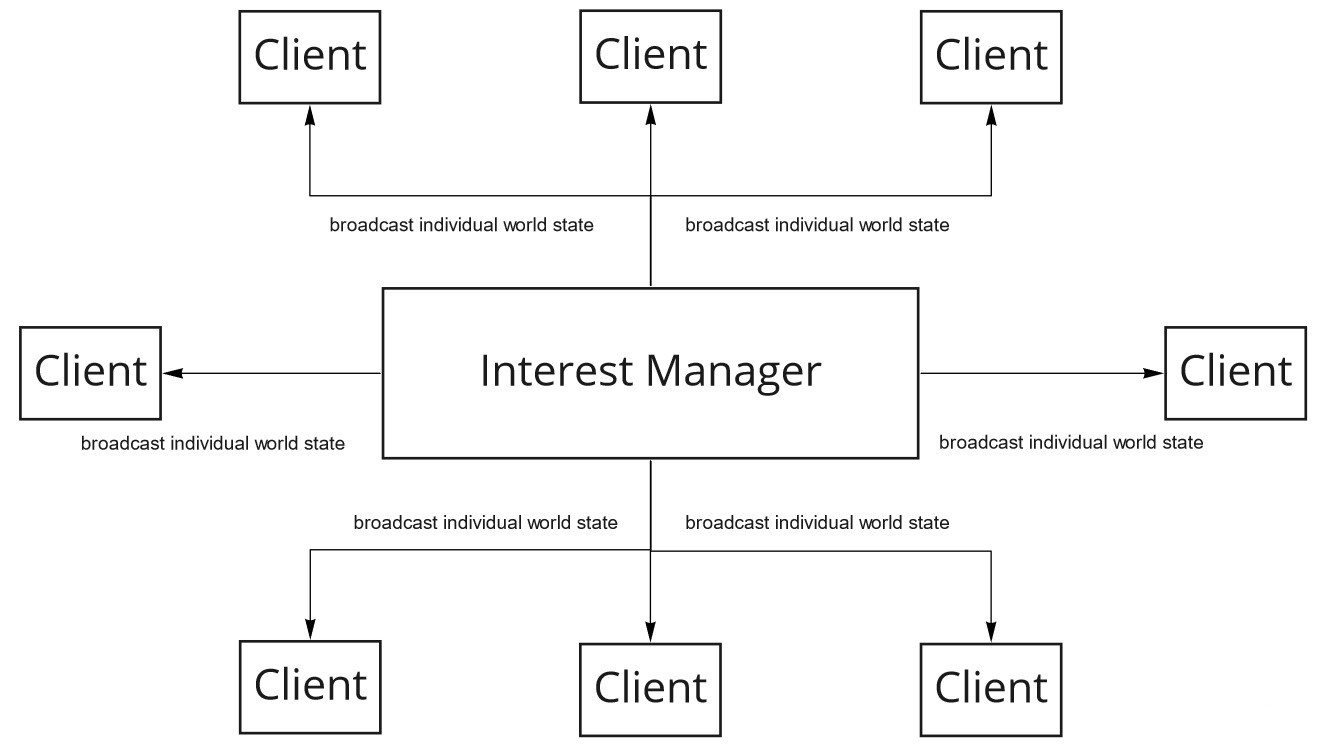
\includegraphics[width=150mm]{images/Interest_Manager.jpg}
	\caption[Interest Manager]{Veranschaulichung des Interest Manager Konzepts}
	\label{pic:Interest_Manager}
\end{figure}

Mögliche Faktoren, die der Interest Manager benutzen kann, um den Spielern die Objekte anzeigen zu lassen, die sie sehen dürfen sind:

- Distanz zwischen Spieler und anderen Objekten

- Teams bzw. Gruppen. Die registrierten (Spieler)-Objekte innerhalb eines Teams/ einer Gruppe sind für Spieler, welche ebenfalls innerhalb des Teams/Gruppe registriert sind sichtbar.

- Spatial Hashing / Grid Checker: Die Spielwelt und ihre Objekte werden in quadratische Zellen eingeteilt. Je nachdem in welcher Zelle sich ein Spieler befindet, werden nur diejenigen Objekte der Spielwelt mit dem Spieler snychronisiert, welche sich innerhalb der 8 "Nachbarzellen" befinden:

\begin{figure}
	\centering
	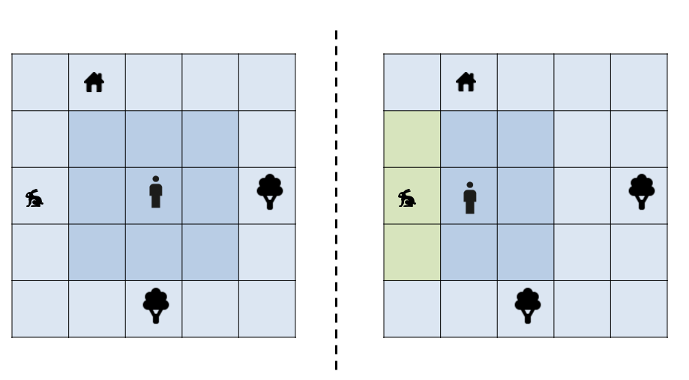
\includegraphics[width=150mm]{images/interest_management.png}
	\caption[Interest Management]{Illustration des Konzepts Interest Management. \cite{JeromeRenaux.2017} }
	\label{pic:interest_management}
\end{figure}

Sollte keine der hier beschriebenen Beispiele auf das gewünschte Spielkonzept passen, so ist es notwendig, eine komplett eigene Logik für das Interest Management zu implementieren.

\section{Studienkonzept}
\label{studienkonzept}

! STUDIENKONZEPT IST NOCH PRE-PRE-ALPHA (enthält Notizen)!

Wie bereits im Teil der Einführung erwähnt, hat diese Arbeit nicht den Anspruch zu beweisen, dass die Konzepte tatsächlich einen Mehrwert für eine Vielzahl an Projekten bieten. Um dies beweisen zu können, ist eine weitere Studie nötig. Im Rahmen dieser Arbeit wurde ein Studienkonzept erarbeitet, welches zukünftig für andere Arbeiten genutzt werden kann.

Das Studienkonzept gliedert sich in:

Repräsentative Umfragen (Umsetzung mit Likert-Skala):
Diese beinhaltet die Befragung von mehreren Hundert Personen aus unterschiedlichen Ländern sowie unterschiedlichen Online-Genres (MMORPG, First Person Shooter, Mobile-Games, etc.).

Folgende Fragestellungen müssen untersucht werden:

Welche Probleme haben angehende Entwickler für Online-Multiplayer Spiele?
Lassen sich diese Probleme auf die in dieser Arbeit beschriebenen Konzepte übersetzen?
Bringen die hier beschriebenen Konzepte einen Vorteil in der Praxis?
	
Zunächst müssen Frage - und Problemstellungen, welche als Annahme getroffen wurden, in Fragen umgewandelt werden. Diese Frage - und Problemstellungen beziehen sich auf konkrete Themen der Multiplayer-Spielenentwicklung.
	
Fragen an junge, angehende Online-Spieleentwickler, welche ein eigenes Projekt umgesetzt haben bzw. welches sich aktuell in Umsetzung befindet:

Problemstellung/Annahme: Es gibt inzwischen viele Frameworks und Engines zur Entwicklung von Online-Multiplayerspielen \cite{MFatihMAR.2021}. Die Entscheidung eine passende Technologie auszuwählen ist mühsam.

Abgeleitete Frage: Wie leicht kamen sie zurecht bei der Auswahl eines Frameworks und/oder eine Game-Engine für ihr erstes Online-Multiplayer Projekt?

Auswahlmöglichkeiten: Auswahl fiel mir sehr leicht, Auswahl fiel mir leicht, Auswahl fiel mir schwer, Auswahl fiel mir sehr schwer

...weitere Fragen...

	--> Umfrage veröffentlichen
	
Die Umfrage soll per Email an ausgewählte Personen an Hochschulen und Unternehmen verschickt werden. Außerdem kann die Umfrage in einschlägige Entwicker-Foren gepostet werden. Beispiele hierfür sind: forum.unity.com , forums.unrealengine.com, www.gamedev.net/forums/forum/8-networking-and-multiplayer.

Die Umfrage kann anonymm, oder mit Personenbezug für eine bessere Auswertung der Ergebnisse erfolgen. Ebenso wäre es denkbar getrennte Umfragen für eine Gruppe an ausgewählten Einzelpersonen sowie die öffentliche Entwickler-Community im Internet zu erstellen.
	
	--> Parallel Versuch starten: 2 Gruppen von Anfänger Entwicklern eine Aufgabe geben (Multiplayer-Spiel bauen), eine bekommt die Konzepte, die andere nicht.
	
	- Control Experiment -> Mehr Beschreiben: Was für Variablen gibt es?
	-> Anforderungen an ein Spiel (Wurde alles erfüllt)
	-> Methodisches Vorgehen
	
Mithilfe eines Experiments (oder mehrerer Experimente) soll gezeigt werden, dass Einstiegs-Entwickler in der Multiplayer-Spieleprogrammierung einen klaren Vorteil haben, wenn sie das technische Design eines Neuprojekts nach diesen Konzepten ausrichten.

Hierfür werden 2 Gruppen aus jeweils maximal 3 Personen bestimmt, welche beide ein identisches, rudimentäres Online-Spiel entwickeln sollen. Die eine Gruppe bekommt die Konzepte als Orientierung zur Verfügung, die andere nicht.

Die Anforderungen an die Probanden sind:
--> Sollten die Probanden aus Studenten bestehen, so müssen alle Probanden im gleichen Semester sein.
--> Die Probanden müssen gleich viel (am besten keine, oder wenig) Erfahrung im Bereich der Multiplayer-Spieleentwicklung haben.

Die Anforderungen an das Experiment sind:
--> Es muss die Zeit gemessen werden, wie viel Stunden jede Gruppe zur Fertigstellung des vorgegebenen Projekts benötigt werden.
--> Alle Probanden müssen Zugang zu ähnlicher Hardware besitzen.
--> Die Gruppen teilen die Aufgaben unter sich auf, und suchen sich selbstständig Frameworks und Engines für das Projekt aus.
--> Im Anschluss müssen beide Gruppen die oben erarbeitete Umfrage ausfüllen.


	--> Ergebnisse der Umfrage auswerten, passen die Ergebnisse zu der hier beschriebenen Problemstellung?

Die Ergebnisse der Umfrage an ausgewählte Personen und an die Entwickler Community werden ausgewertet. Kann man einen Trend erkennen? Können die Problemstellungen / Thesen validiert werden? 
(Konkret: Sind die Annahmen dieser Arbeit korrekt? Haben Anfänger-Entwickler tatsächliche Schwierigkeiten mit den Punkten X, Y, Z ..?)

	--> Auswertung des Experiments / der Experimente: Hat die Gruppe, welche sich an die Konzepte gehalten hat einen messbaren Vorteil gehabt? (Geschwindigkeit, Anfangsschwierigkeiten)
	
Die Daten aus dem Experiment (Zeitmessung, Umfrageergebnisse) sollen nun wie folgt ausgewertet werden:

--> Ist die Gruppe, welche das Projekt mit den Konzepten umgesetzt hat, schneller zum Ziel gekommen, als die Gruppe ohne Hilfestellung der Konzepte?

--> Hatte die Gruppe, welche das Projekt mit den Konzepten umgesetzt hat, weniger Start-Schwierigkeiten bei der Umsetzung des Projekts, als die Gruppe ohne Hilfestellung der Konzepte?


Weitere Punkte, die in Studienkonzept noch fehlen:
--> Methodik für semi-strukturiertes Experteninterviews beschreiben







